\documentclass[a4paper,10pt]{article}

\usepackage[utf8]{inputenc}
\usepackage[english]{babel}
\usepackage[T1]{fontenc}
\usepackage{palatino}

\usepackage[colorlinks=true]{hyperref}
\hypersetup{urlcolor=black,linkcolor=black}

\usepackage{enumerate}

\usepackage{fullpage}
\setlength{\parindent}{0pt}
\setlength{\parskip}{\medskipamount}

\usepackage{amsmath}
\usepackage{amssymb}
\usepackage{mathrsfs}
\usepackage{amsthm}
\usepackage{array}
\usepackage{graphicx}


\title{Project proposal}
\author{PPP \--- ENS Lyon}
\date{M1. 2014}

\begin{document}
\maketitle

\begin{tabular}{|ll|}
\hline
Title & Projet Pensées Profondes (PPP)\\
Coordinator & Marc \textsc{Chevalier}\\
Members & Raphaël \textsc{Charrondière}, Marc \textsc{Chevalier}, Quentin \textsc{Cormier}, \\
        & Tom \textsc{Cornebize}, Yassine \textsc{Hamoudi}, Valentin \textsc{Lorentz},\\
        & Thomas \textsc{Pellissier} \textsc{Tanon}\\
\hline
\end{tabular}

\section{Expected results}
\emph{What is the birth date of the first president of the United States?} This is
the typical question that we would like to answer automatically.

This requires three steps. 

Firstly, understanding the natural language. The input string given in standard 
English has to be transformed into a normal form. To do so, we will use natural 
language processing (NLP) libraries. We will also implement a machine learning (ML)
algorithm, in order to improve the answers of our software.

Then, the normal form is used to collect data, by querying some data base (e.g.
Wikidata). Some operations may then be applied, like performing a sort.

Finally, the desired answer is displayed.


\section{Technological innovations}

\section{Concurrent services}

Several private companies offer question answering frameworks. 

WolframAlpha \footnote{\url{https://www.wolframalpha.com/}}, a tool developed by 
Wolfram Research, provide a web based service to answer directly to questions asked
in English. It is well known for its abilities to process mathematical statements.
It focuses on historical and scientific facts, such as \emph{When was the French 
revolution?} or \emph{What is the root of pi?}.

Google Now \footnote{\url{http://www.google.com/landing/now/}} and Siri
\footnote{\url{https://www.apple.com/fr/ios/siri/}}, two intelligent personal assistants
developed respectively by Google and Apple, provide a mobile based service to 
answer questions asked in natural language (generally, those of the owner of the
mobile device). They focus on practical facts, such as \emph{Where is the nearest
restaurant?}.

In a first time, the PPP project aims to provide a clever way to browse Wikidata, by giving the 
user the direct answer to his question, not the link of the related Wikipedia
web page. Thus, our software will not be suited to answer such practical questions,
although some new modules can be made if there exists a related database. Google Now
and Siri are therefore not direct concurrent services.

The PPP project is closer to the WolframAlpha tool. However, it is a free project,
and will be modular and well documented. We hope that it will interest the 
Wikipedia community, in order to keep it updated in the future. Moreover,
we will not focus on mathematical questions, as WolframAlpha does.


\section{Software}

The goal is to develop a query answering framework able to answer to simple questions with different back-end. 

\begin{figure}[!h]
    \centering
    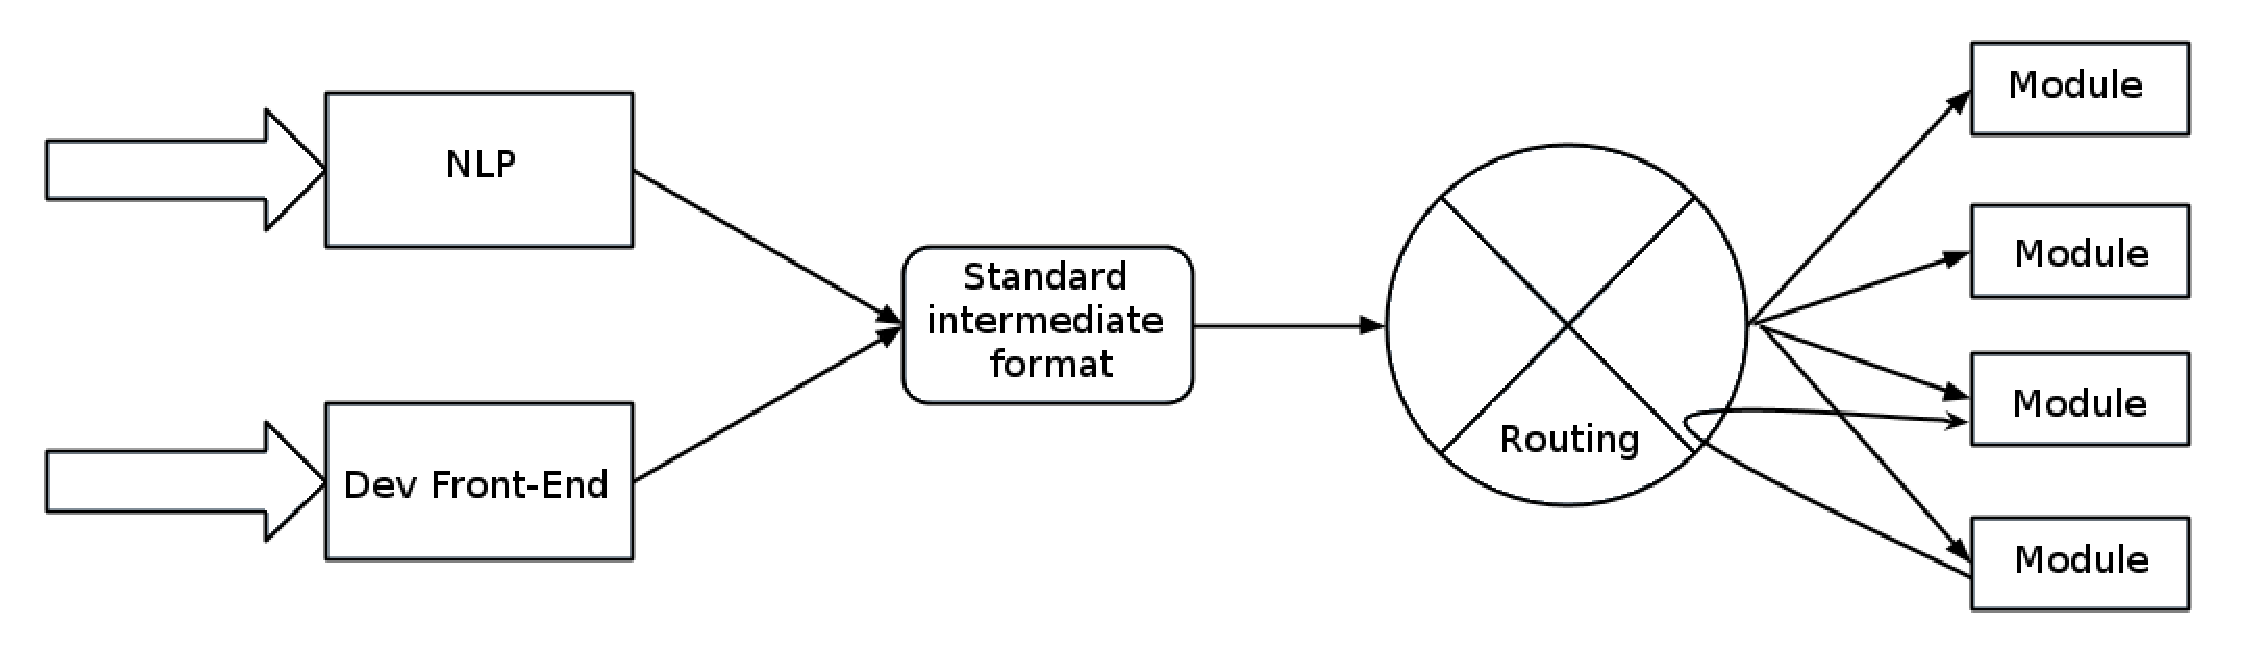
\includegraphics[scale=0.39]{images/Structure-PPP-en.eps}
    \caption{Global structure}
\end{figure}

\section{Target public}

The first goal of the PPP project is to provide a free, modular and well documented search engine tool that will 
interest research communities for extensibility features. Our purpose is to allow people to design their own modules and
easily include them in the tool. For example, sports modules could be done to answer questions about contests results or 
upcoming meetings. We intend to make at least one module, using Wikidata, in order to provide a demo and attract the big 
community of Wikidata. 

On the other hand, we also target the potentially users of our tool. We hope to provide a clever, transparent and easy to use search 
engine tool that will convince people of its utility. At a time when intelligent search engine tools are increasingly used, we think it is
now or never for the open source community to propose its own product.

\section{Schedule}

\section{Task partition}

\section{Organization}

% \section{Budget} not necessary to make a part to explain that there is no budget... just say it in Organization section


\end{document}

